
\documentclass[xcolor=x11names,compress]{beamer}

% Many thanks to http://cameron.bracken.bz/beamer-template
%% General document %%%%%%%%%%%%%%%%%%%%%%%%%%%%%%%%%%
\usepackage{graphicx}
%%%%%%%%%%%%%%%%%%%%%%%%%%%%%%%%%%%%%%%%%%%%%%%%%%%%%%


%% Beamer Layout %%%%%%%%%%%%%%%%%%%%%%%%%%%%%%%%%%
\useoutertheme[subsection=false,shadow]{miniframes}
\useinnertheme{default}
\usefonttheme{serif}
\usepackage{palatino}

\setbeamerfont{title like}{shape=\scshape}
\setbeamerfont{frametitle}{shape=\scshape}

\setbeamercolor*{lower separation line head}{bg=DeepSkyBlue4} 
\setbeamercolor*{normal text}{fg=black,bg=white} 
\setbeamercolor*{alerted text}{fg=red} 
\setbeamercolor*{example text}{fg=black} 
\setbeamercolor*{structure}{fg=black} 
 
\setbeamercolor*{palette tertiary}{fg=black,bg=black!10} 
\setbeamercolor*{palette quaternary}{fg=black,bg=black!10} 

\renewcommand{\(}{\begin{columns}}
\renewcommand{\)}{\end{columns}}
\newcommand{\<}[1]{\begin{column}{#1}}
\renewcommand{\>}{\end{column}}
%%%%%%%%%%%%%%%%%%%%%%%%%%%%%%%%%%%%%%%%%%%%%%%%%%










% \usetheme{Malmoe}
% \usetheme{Luebeck}
% \usetheme{Antibes}
% \usecolortheme{rose}
\usepackage{graphicx}
\DeclareGraphicsExtensions{.pdf,.png,.jpg}
\graphicspath{{./images/}}
\usepackage{hyperref}
\usepackage{color}
% ---------------------------------------------------------------------------------------
% Thanks to http://www.guidodiepen.nl/2009/07/creating-latex-beamer-handouts-with-notes/
 % \usepackage{handoutWithNotes}
 % \pgfpagesuselayout{4 on 1 with notes}[a4paper,border shrink=5mm]
 % \pgfpagesuselayout{2 on 1 with notes landscape}[a4paper,border shrink=5mm]
% ---------------------------------------------------------------------------------------

\title{Mazes: An Introduction}
\author{Stephen Wattam}
\institute[2012]{Computing Society of Lancaster University}
\date{\tiny November 1st, 2012}

\begin{document}

\frame{\titlepage}

\section[Outline]{}
\frame{\tableofcontents}

% -----------------------------------------------------------------------------------------
\section{Overview}
\subsection{What is a Maze?}
\frame{\frametitle{What is a Maze?}
\begin{columns} 
    \begin{column}[c]{5cm} 

        \begin{itemize}
            \item<1-> A space with walls
            \item<2-> Has a start and finish (or entrance/exit)
            \item<3-> Stops you from finding your bone

            \item<4-> \textbf{Has some feature making it hard to follow the path}
        \end{itemize}
    \end{column} 
\begin{column}[c]{5cm} 

    \begin{center}
        \includegraphics<3->[width=5cm]{sparky}
    \end{center}

\end{column} 
\end{columns}

\note{Here are some more insulting comments that I wish to make.  
The class will not see them on the overhead, but I will see them on my 
laptop.}
}



\subsection{Types of Maze}
\frame{\frametitle{Perfect}
\begin{itemize}
    \item<1-> Has no loops
    \item<2-> Has a route to every point in the maze
\end{itemize}
\begin{center}
    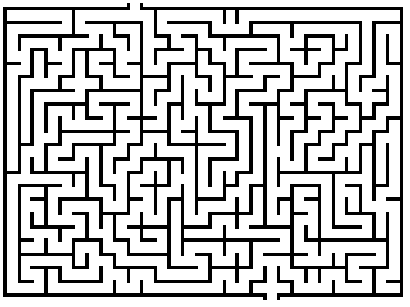
\includegraphics[width=5cm]{perfect}
\end{center}
}
\frame{\frametitle{Braid}
\begin{itemize}
    \item<1-> Has no dead ends, instead using passages that run around and join up again
    \item<2-> Much harder to solve (and generate!)
\end{itemize}
\begin{center}
    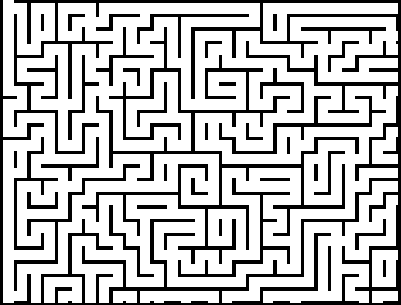
\includegraphics[width=5cm]{braid}
\end{center}
}
\frame{\frametitle{Unicursal}
\begin{itemize}
    \item<1-> Has no junctions, so is a single path
    \item<2-> Sometimes called a labyrinth
    \item<3-> Trivial to solve with automated means
\end{itemize}
\begin{center}
    
\includegraphics[width=5cm]{unicursal}
\end{center}
}
\frame{\frametitle{Sparse}
\begin{itemize}
    \item<1-> Wide, irregularly-spaced passages.
    \item<2-> Often come in cool designs (not shown here).
\end{itemize}
\begin{center}
    
\includegraphics[width=5cm]{sparse}
\end{center}
}

\subsection{Properties of Mazes}
\frame{\frametitle{Properties of Mazes}
\begin{itemize}
    \item<1-> \textbf{Bias}---The tendency of a maze to have horizontal or vertical passages.  Makes it hard to go `against the grain'
    \vspace{15pt}
    \item<2-> \textbf{Run}---A long, straight, uninterrupted passage
    \vspace{15pt}
    \item<3-> \textbf{Elitism}---The ratio of the maze's shortest path against its total path length
\end{itemize}
}


% -----------------------------------------------------------------------------------------
\section{Mice}
\subsection{What's one of thems?}
\frame{\frametitle{Mice}

\begin{columns} 
    \begin{column}[c]{8cm} 

\begin{itemize}
    \item<1-> Mice are \textbf{Maze-solving robots}\\
        \visible<2->{\small Mice are also mice}
    \vspace{10pt}
    \item<3-> Compete in many competitions, solving real-life mazes {\tiny (\href{http://www.youtube.com/watch?v=_L9rkLAskWU}{Click me!})}
    \vspace{10pt}
    \item<4-> Limited view of the maze, limited processing power
    \vspace{10pt}
    \item<5-> No awareness of the maze other than what is learned
\end{itemize}

    \end{column} 
\begin{column}[c]{3cm} 

    \begin{center}
        \includegraphics<2->[width=3cm]{mouse1}\\
        \vspace{12pt}
        \includegraphics<1->[width=3cm]{mouse2}
    \end{center}

\end{column} 
\end{columns}
}


\subsection{Abilities \& Limitations}
\frame{\frametitle{Abilities \& Limitations}
\begin{columns} 
    \begin{column}[c]{7cm} 

\begin{itemize}
    \item<1-> Solving a maze is easy, if you can see it all
        \visible<2->{\tiny (\href{http://www.funnyordie.com/videos/2fe034255a/trapped-in-hedge-maze-from-stevanhogg\%20\%5B+\%5D}{Click me!})}
    \vspace{15pt}
    \item<3-> Mice rely only on pactical real-world input from sensors
    \vspace{15pt}
    \item<4-> So how do they do it? 
\end{itemize}

    \end{column} 
\begin{column}[c]{4cm} 

    \begin{center}
        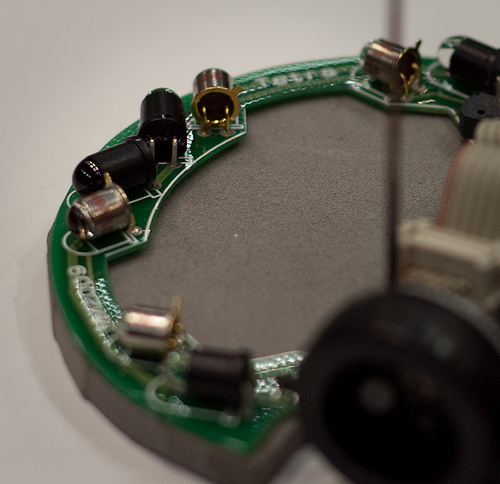
\includegraphics[width=4cm]{mouse3}
    \end{center}

\end{column} 
\end{columns}
}





% -----------------------------------------------------------------------------------------
\section{Control Theory \& Agent-based AI}
\subsection{Overview, Sensing and Actuating}
\frame{\frametitle{Measure--Model--Respond}
\begin{itemize}
    \item<1-> Similar to control theory---each mouse is an `intelligent agent', judging the state of the world from its inputs
    \item<2-> Three basic stages, repeated \textsl{ad infinitum}:
        \begin{enumerate}
            \item<3-> \textbf{Measure} the world about you;
            \item<4-> \textbf{Model} the rest of it to create a virtual world;
            \item<5-> \textbf{Respond} by using information from the model.
        \end{enumerate}
\end{itemize}

\begin{center}
    \includegraphics<3->[width=8cm]{control}
\end{center}

}

\frame{\frametitle{Measure--Model--Respond Problems}
\begin{itemize}
    \item<1-> \textcolor<5->{gray}{Sensors are often inaccurate, or tell us confusing, simple things (data is not information)}
    \item<2-> \textcolor<5->{gray}{The world changes, even when we're not the ones changing it}
    \item<3-> \textcolor<5->{red}{Modelling even simple worlds is difficult!}
    \item<4-> \textcolor<5->{red}{We have to know what to do, even if our model is incomplete}
\end{itemize}
\begin{center}
    \visible<5->{The items in red are all you have to worry about in Maize.}
\end{center}
}


\subsection{Types of Agent}
\frame{\frametitle{Managing the World}
    \begin{itemize}
        \item<1-> \textbf{Stateful/Stateless}---Do we want to remember past events, or treat each sensor reading as a new event?
        \vspace{10pt}
        \item<2-> \textbf{Deterministic/Stochastic}---Do we want to respond in a purely predictable manner?
        \vspace{10pt}
        \item<3-> \textbf{Discrete/Continuous}---Are all of our values smoothly variable? Can we react partially/smoothly?
    \end{itemize}
}
\frame{\frametitle{Inferring State---FSMs}
    \begin{itemize}
        \item<1-> Display how the world \textbf{is}, based on how it \textbf{has changed}
        \item<2-> Can be interrogated without needing new sensor data
        \item<3-> Make transitions between states based on arbitrary, even probabalistic, rules
        \item<4-> Underpin all of computing!
    \end{itemize}

\begin{center}
    \includegraphics<3->[width=8cm]{fsm}
\end{center}
}
\frame{\frametitle{Determinism}
    \begin{itemize}
        \item<1-> Given the same (sequence of) input, will \textbf{always} produce the same output
        \vspace{10pt}
        \item<2-> Very reliable\\
            \visible<3->{\small but also reliably bad if the rules are poor}
        \vspace{10pt}
        \item<4-> Nondeterminism can involve fuzzy logic, probability, or guesswork\\
            \visible<5->{\small Closer to human judgement, but very hard to get `just right'}
    \end{itemize}
}
\frame{\frametitle{Discrete \& Continuous Control}
    \begin{itemize}
        \item<1-> Continuous control allows for small tweaks and improvements
        \vspace{10pt}
        \item<2-> Can be hard to rationalise logically---needs threshold values or statistics
        \vspace{10pt}
        \item<3-> Can offer better control and progressive feedback\\
            \visible<4->{\small Confident bots can rush quickly; Unsure ones can creep to gather more information}
    \end{itemize}
}
\frame{\frametitle{Demos}
    \begin{itemize}
        \item<1-> Deterministic vs. Stochastic
        \begin{itemize}
            \item<2-> DaveBot is stochastic, has no rules
            \item<2-> LeftBot is deterministic, has only rules
        \end{itemize}

        \vspace{10pt}
        \item<3-> Discrete vs. Continuous
        \begin{itemize}
            \item<4-> LeftBot is discrete, one move per assessment
            \item<4-> AdvancedBot has some continuous properties: command queueing
        \end{itemize}

        \vspace{10pt}
        \item<5-> Stateful vs. Stateless
        \begin{itemize}
            \item<6-> LeftStateBot is stateful, remembers a long sequence of actions
            \item<6-> LeftBot is not
        \end{itemize}
    \end{itemize}
}

\subsection{Limits to Computability}
\frame{\frametitle{Complexity of Maze Solving}
    \begin{itemize}
        \item<1-> Algorithmically, the best solution to a maze is to choose the best right path each time:\\
            \textcolor<2->{red}{The maze is just a big tree of choices}
        \vspace{10pt}
        \item<3-> The best case is thus equivalent to a binary search, plus the time needed to move
        \vspace{10pt}
        \item<4-> This becomes $O(n log_2 n)$, where $n$ is the number of choices (plus a bit of time to travel from start to finish).
    \end{itemize}
}




% -----------------------------------------------------------------------------------------
\section{Introduction to Maize}
\subsection{The Framework}
\frame{\frametitle{Overview}
    \begin{itemize}
        \item<1-> Manages \texttt{Bot}s and \texttt{Maze}s, and simulates a virtual world
        \item<2-> Tile-based environment
        \item<3-> A tile can be a start, finish, space, or wall.
    \end{itemize}


\begin{center}
    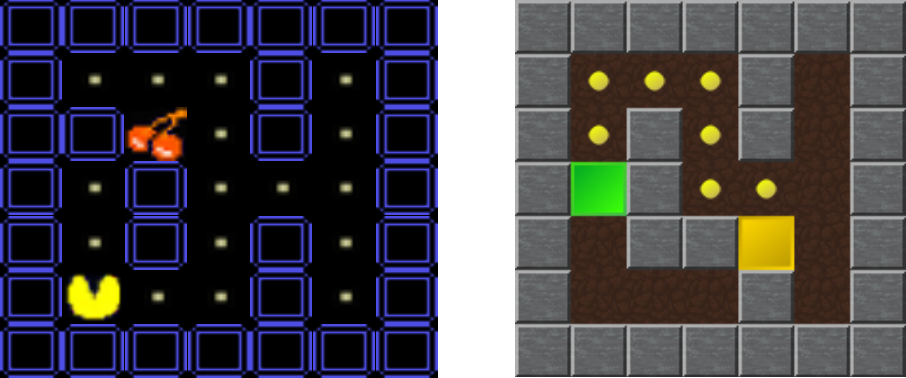
\includegraphics[width=3cm]{mazepic1}
\end{center}
}
\frame{\frametitle{The Life of a Bot}
    \begin{itemize}
        \item<1-> Bots get restricted data:
            \begin{itemize}
                \item<2-> \textcolor<6->{red}{Their immediate surroundings (3x3 array around them)}
                \item<3-> \textcolor<6->{gray}{Bot co-ordinates in the maze}
                \item<4-> \textcolor<6->{gray}{Bot orientation}
                \item<5-> \textcolor<6->{gray}{Finish point co-ordinates}
            \end{itemize}\\
            \visible<6->{\tiny (Technically, all that's needed is the red one, but the other things make it more fun)}
        \vspace{15pt}
        \item<7-> Bots can move only one tile per `tick', and only Left, Right, Forward and Back (like kings in chess)
    \end{itemize}
}
\frame{\frametitle{Bot Classes}
    \begin{itemize}
        \item<1-> \textbf{Bot}\\
            \begin{itemize}
                \item<2-> Simplest API available
                \item<3-> Maize calls \texttt{nextMove()} on every tick.
                \item<4-> Simply return a direction to move.
            \end{itemize}
        
        \vspace{10pt}
        \item<5-> \textbf{AdvancedBot}\\
            \begin{itemize}
                \item<6-> Like \texttt{Bot}, but only requests a move when it has emptied its queue
                \item<7-> Has a queue commands can be added to, and a more powerful high-level API (\texttt{moveLeft()}, \texttt{turnRight()} etc)
            \end{itemize}
    \end{itemize}
}
\subsection{Code Introduction}
\frame{\frametitle{Demo, Code Rundown}
    \begin{center}
        A quick overview of the bots we have\\
        \vspace{10pt}
        \url{http://extremetomato.com/projects/maize/}
    \end{center}
}
% -----------------------------------------------------------------------------------------
\section{Challenges}
\frame{\frametitle{Challenges}
    \begin{enumerate}
        \item<1-> Beat \texttt{DaveBot} on any Maze\\
            {\small (An \texttt{EmptyMaze} might be simplest, a \texttt{ScatterMaze} might be hardest)}
        \vspace{5pt}
        \item<2-> Solve a DFS Maze without using a wall following algorithm\\
            {\small (this requires building a model of the decision tree)}
        \vspace{5pt}
        \item<3-> Write a wall follower that can also solve \texttt{Empty} and \texttt{Scatter} mazes.
        \vspace{5pt}
        \item<4-> Improve an existing wall follower with heuristics
    \end{enumerate}
}
\frame{\frametitle{Getting Started (abstract)}
    \begin{itemize}
        \item<1-> Decide on a maze type to run on
        \vspace{10pt}
        \item<2-> Decide on a strategy to try
        \vspace{10pt}
        \item<3-> Code, or pair up with someone who wishes to, and hack at it
        \vspace{10pt}
        \item<4-> Submit to \texttt{stephenwattam@gmail.com} for a glorious battle, with prizes if I can be arsed.
    \end{itemize}
}
\frame{\frametitle{Getting Started (concrete)}
    \begin{itemize}
        \item<1-> Create a new class in \texttt{./bots/} that \texttt{extends Bot}
        \vspace{10pt}
        \item<2-> Start Maize.  Compiler output will be in the console.
        \vspace{10pt}
        \item<3-> Edit your bot and select \texttt{Bots > Reload all Bots} or \texttt{Bots > Compile} to recompile.
        \vspace{10pt}
        \item<4-> The log contains compiler output from your bots.
    \end{itemize}
}

\frame{\frametitle{Fin}
    \begin{center}
        All resources available from\\
        \vspace{10pt}
        \url{http://extremetomato.com/projects/maize/}
    \end{center}
}


% -----------------------------------------------------------------------------------------
\end{document}
